\documentclass[a4paper]{article}
\usepackage[utf8]{inputenc}
\usepackage[russian]{babel}
\usepackage[dvips]{graphicx}
%\usepackage{mathtext}
\usepackage{amsmath}
\usepackage{indentfirst}  % абзацный отступ после заголовка
\usepackage{misccorr}  % точка в заголовке
\usepackage{longtable}
\usepackage{verbatim}  % текст программы

\usepackage{setspace}  % интервалы
\onehalfspacing % полутроный интервал

\usepackage{geometry}  % установка полей
\geometry{top=3.5cm,bottom=2cm,left=2cm,right=2cm}

\parindent=15mm
%\frenchspacing  % без пробелов после предложений

\usepackage{fancyhdr}  % колонтитулы
\pagestyle{fancy}  % смена стиля оформления страниц
\fancyhf{}  % очистка текущих значений
%\fancyhead[C]{\thepage}  % верхний колонтитул
\fancyhead[C]{\fontsize{14pt}{18pt}\selectfont\thepage}  % верхний колонтитул 
\renewcommand{\headrulewidth}{0pt}  % убрать разделительную линию 

\begin{document}
\begin{titlepage}
\begin{center}

\fontsize{14pt}{18pt}
\selectfont

\vfill
Федеральное агентство по образованию РФ\\
Новгородский государственный университет им.~Ярослава~Мудрого

\hrulefill

Кафедра ИТИС

\vfill
\vfill

{
\huge
Реализация алгоритмов поиска корней~уравнений\linebreak
методом половинного деления и методом хорд
}

\vfill

{
\begin{flushright}
Выполнил студент группы 9311\\
Лопатин А.С.
\end{flushright}
}

\vfill

Великий Новгород, 2009
\end{center}
\end{titlepage}

\setcounter{page}{2}  % продолжаем со 2-й страницы
\fontsize{14pt}{18pt}\selectfont

\section{Цель работы}
Реализовать алгоритмы численного интегрирования методом трапеций и методом
Симпсона на языке программирования C++.

\section{Математическая модель решения}
Даны границы интегрирования $a$ и $b$, точность $\varepsilon$ и количество узлов
интерполяции $n$.
Требуется найти определенный интеграл $\int\limits_a^b f(x)dx$
(где $f(x)$, например, квадратичная функция $y=10x-2x^2$) численными методами:
методом трапеций и методом Симпсона.

Метод трапеций заключается в замене площади фигуры площадями прямоугольных
трапеций, которые можно вписать в такую фигуру.
Возьмем за длину шага между трапециями
$h=\frac{b-a}{n}$, которая будет также являться ее высотой.
Тогда прямая, проходящая через координаты $(x_i, 0)$ и $(x_i, f(x_i))$ будет
одним из оснований этой трапеции.
Второе же основание будет таким же, но с $x_{i+1}$.
Отсюда можно найти площадь трапеции с помощью полусуммы оснований,
умноженной на высоту: $S_i=\frac{f(x_i)+f(x_{i+1})}{2}\cdot h$.
Остается только просуммировать эти площади:
$$S=\sum_{i=0}^n\frac{f(x_i)+f(x_{i+1})}{2}\cdot h$$
Проверять точность можно просто сравнивая модуль разности предыдущего
результата и текущего с $\varepsilon$.

Метод Симпсона же заключается в замене подынтегральной функции параболой,
которая проходит через три точки отрезка интегрирования
(в качестве таких точек используют концы отрезка и его среднюю точку).
Формула в таком случае выглядит так:
$$S=\frac{b-a}{6}\left(f(a)+4f\left(\frac{a+b}{2}\right)+f(b)\right)$$
Если разбить интервал интегрирования на $2n$ равных частей, то получится:
$$S=\frac{h}{6}
(
    f_0
    + 2(f_2 + f_4 + \ldots + f_{2n-2})
    + 4(f_1 + f_3 + \ldots + f_{2n-1})
    + f_{2n}
)$$
где $f_i=a+\frac{h\cdot i}{2}$.
Проверять точность на соответствие $\varepsilon$ можно по следующей формуле:
$$|S_{j-1}-S_j| > \frac{\varepsilon\cdot h\cdot n}{b-a}$$
где $S_j$ и $S_{j-1}$ площади текущей и предыдущей фигуры соответственно.

\section{Спецификация}
Таблица переменных:
{
\fontsize{10pt}{12pt}\selectfont
\begin{longtable}{|p{1.5cm}|l|p{2.5cm}|l|p{2cm}|p{4.5cm}|}
\hline
Исходное значение & Идентификатор & Тип & Вид & Размерность & Назначение\\
\hline
$a$ & a & Вещественный & Простой & -- & Граница интегрирования\\
\hline
$b$ & b & Вещественный & Простой & -- & Граница интегрирования\\
\hline
$\varepsilon$ & eps & Вещественный & Простой & -- & Точность\\
\hline
$n$ & n & Целый & Простой & -- & Количество узлов\\
\hline
$h$ & h & Вещественный & Простой & -- & Шаг между узлами\\
\hline
$s$ & s & Вещественный & Простой & -- & Сумма\\
\hline
s\_old & s\_old & Вещественный & Простой & -- & Предыдущая сумма\\
\hline
$s_1$ & s1 & Вещественный & Простой & -- & Первая сумма для метода Симпсона\\
\hline
$s_2$ & s2 & Вещественный & Простой & -- & Вторая сумма для метода Симпсона\\
\hline
$x$ & x & Вещественный & Простой & -- & Аргумент функции $f(x)$\\
\hline
$i$ & i & Целый & Простой & -- & Счетчик итераций\\
\hline
done & done & Логический & Простой & -- & Признак соответствия точности\\
\hline
\end{longtable}
}

\newpage
\section{Алгоритм}
\subsection{Функция <<$f(x)$>>}
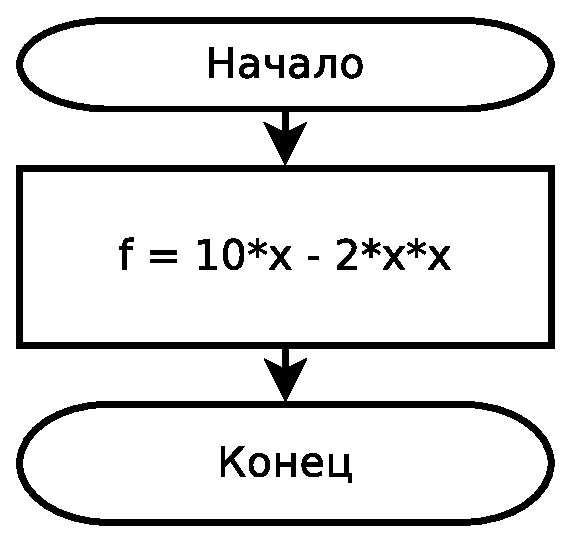
\includegraphics[scale=0.35]{schemes/f}

\subsection{Функция <<$f_i$>>}
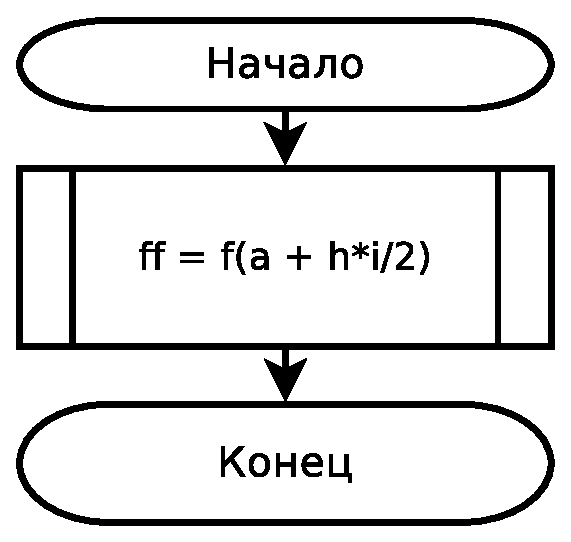
\includegraphics[scale=0.35]{schemes/ff}

\subsection{Функция <<main>>}
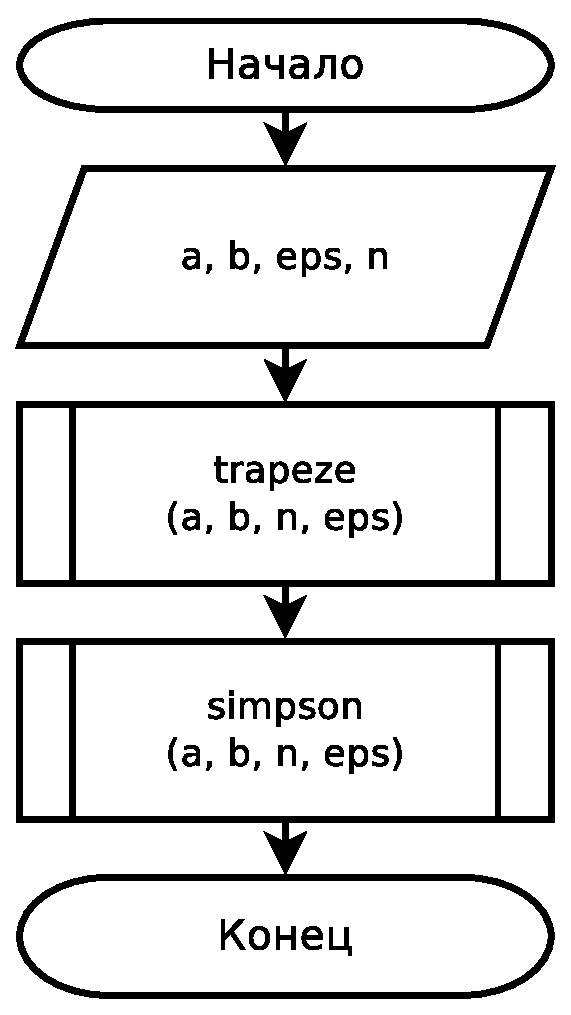
\includegraphics[scale=0.35]{schemes/main}

\subsection{Процедура <<trapeze>>}
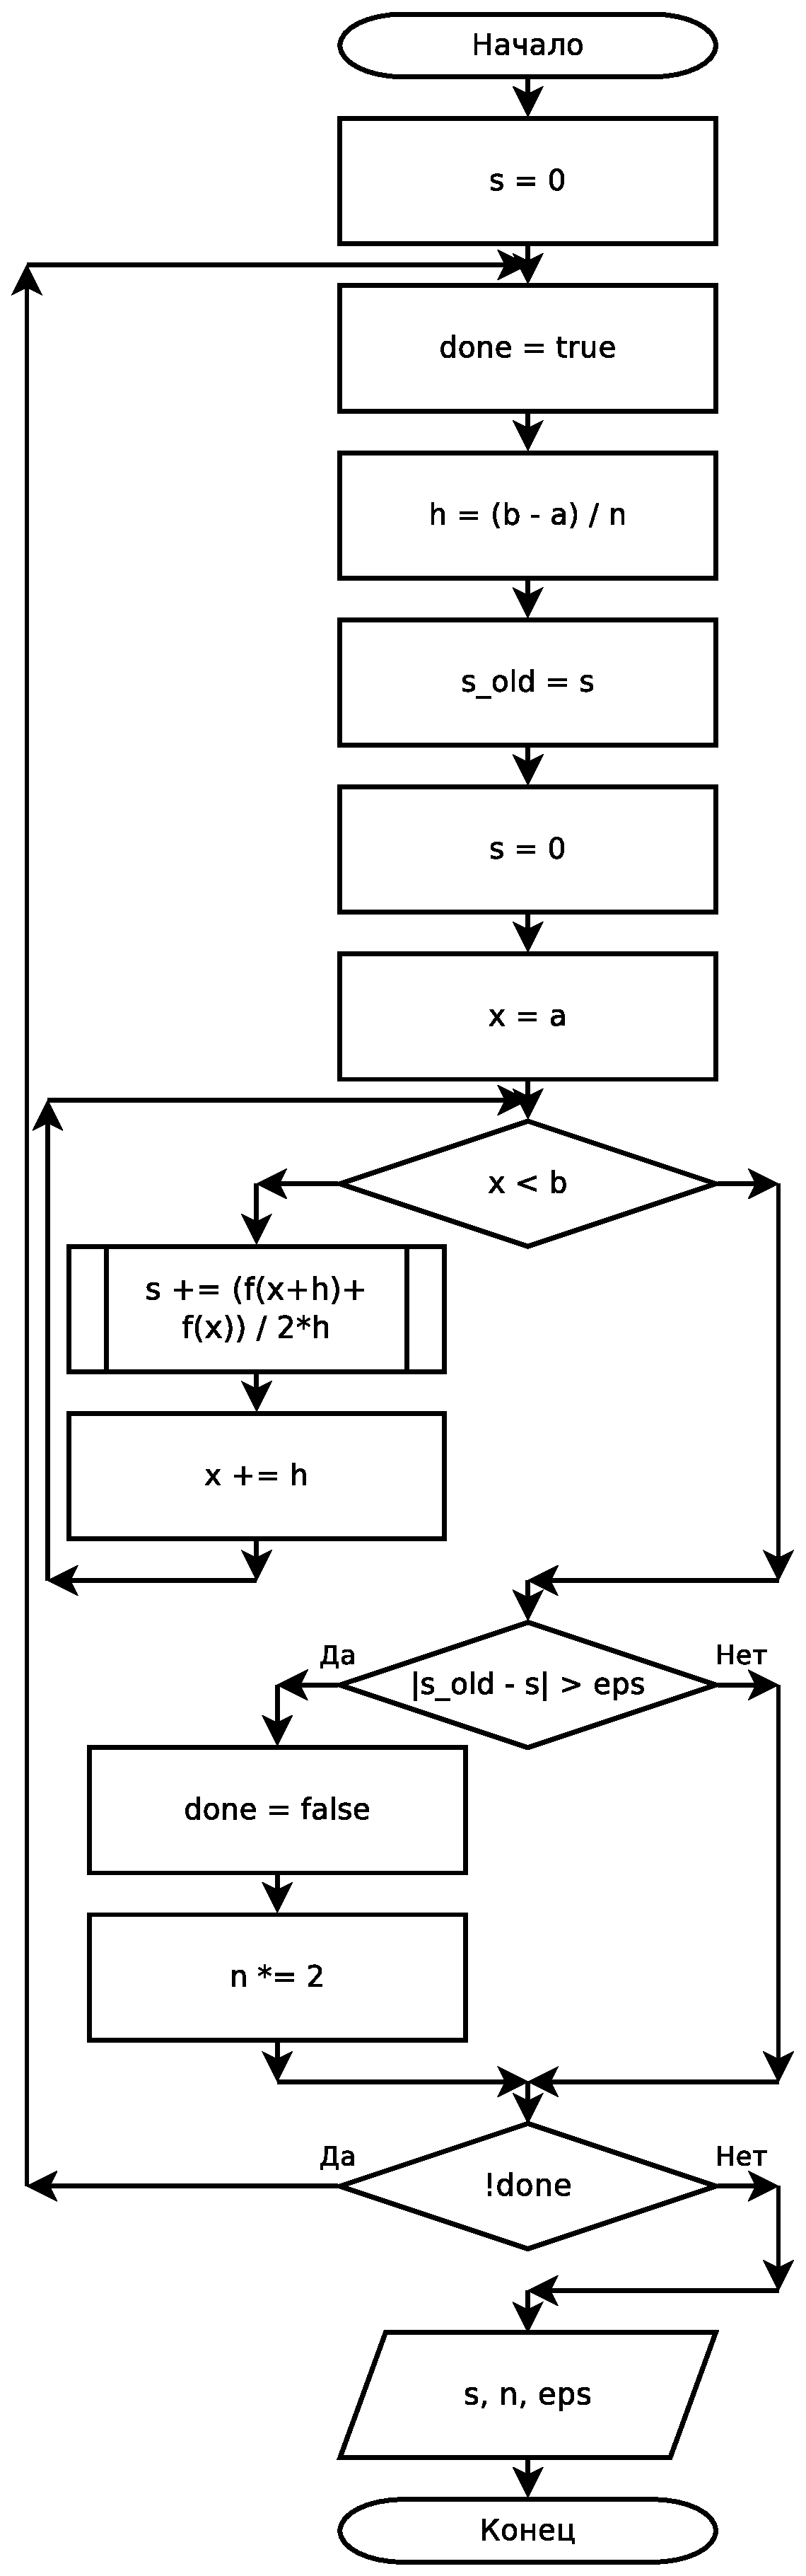
\includegraphics[scale=0.35]{schemes/trapeze}

\subsection{Процедура <<simpson>>}
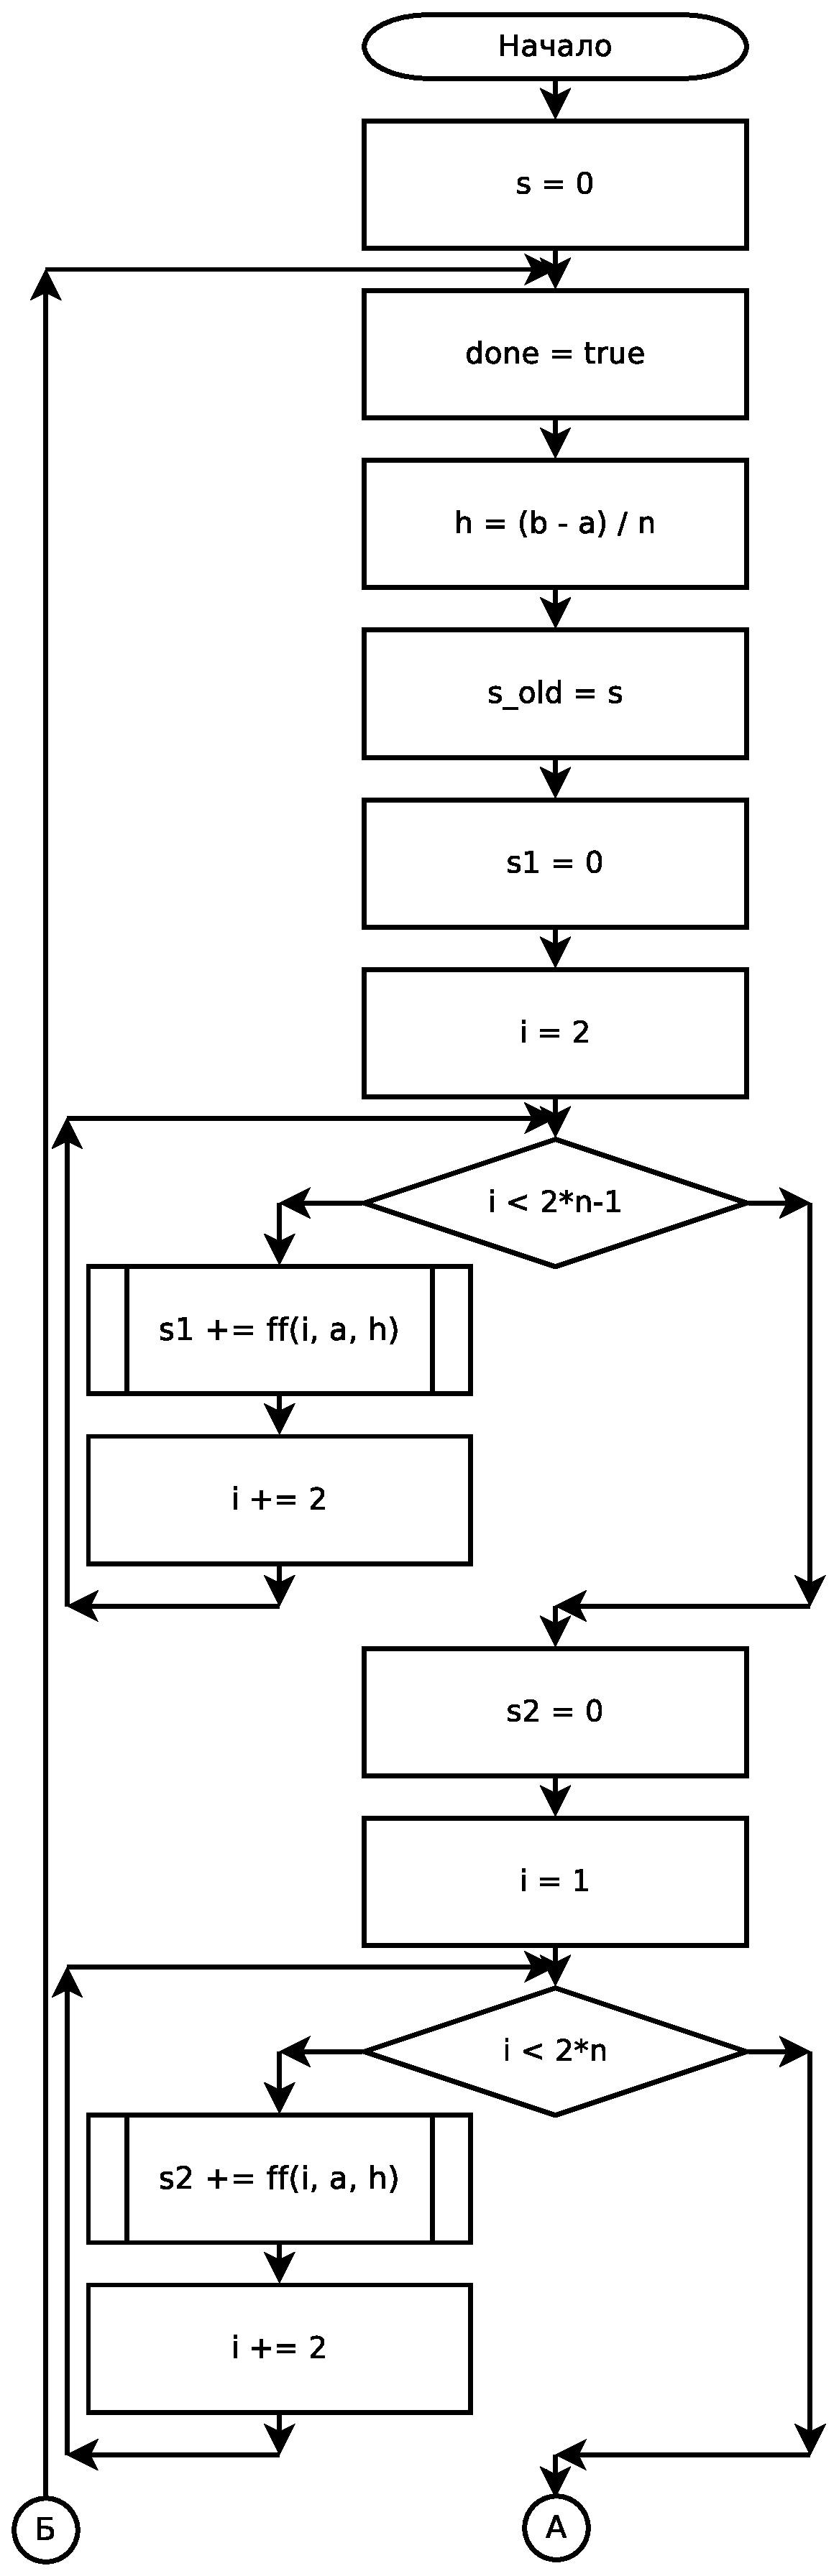
\includegraphics[scale=0.35]{schemes/simpson1}
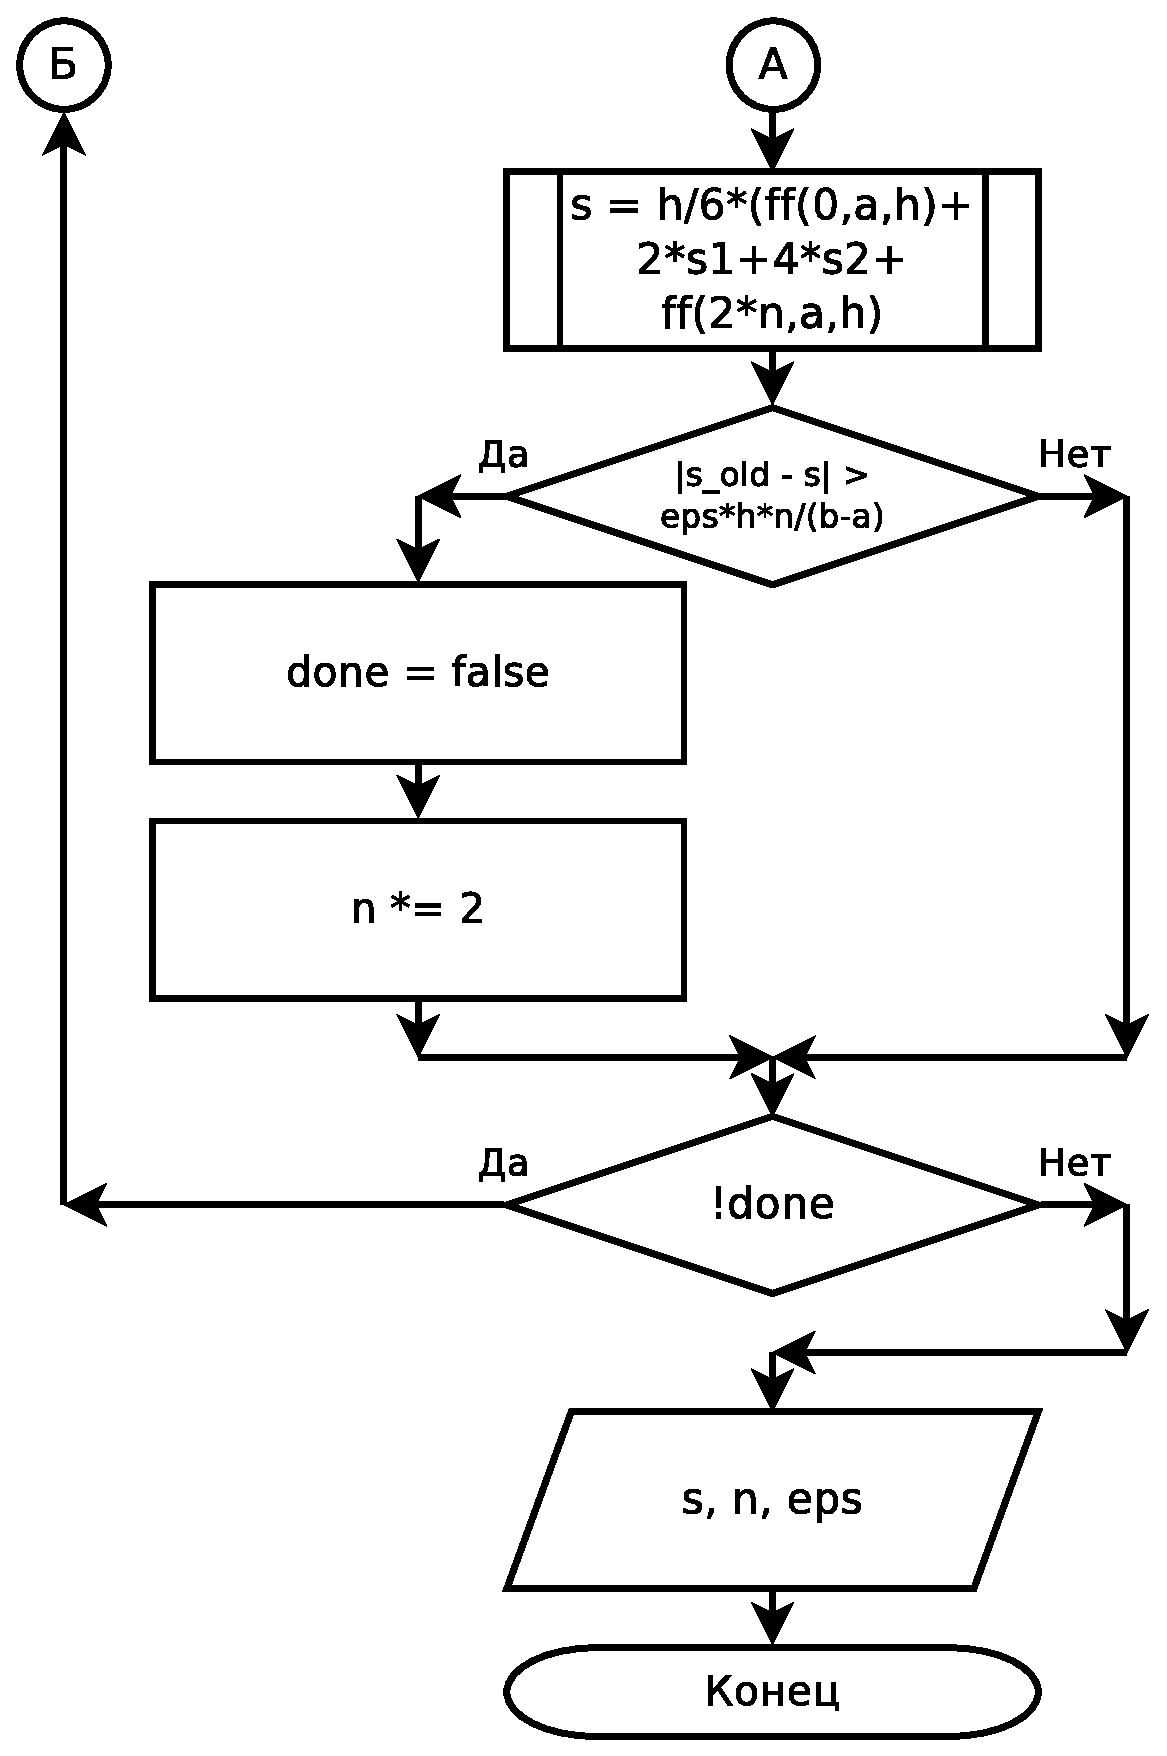
\includegraphics[scale=0.35]{schemes/simpson2}

\section{Программа}
{
\fontsize{12pt}{14pt}
\selectfont
\verbatiminput{../3.cc}
}

\section{Шаблон ввода исходных данных}
{
\fontsize{12pt}{14pt}
\selectfont
\begin{verbatim}
1
10
0.034
34
\end{verbatim}
}

\section{Шаблон вывода результата}
{
\fontsize{12pt}{14pt}
\selectfont
\begin{verbatim}
Trapeze method: s = -171.003, n = 272, eps = 0.034
Simpson's method: s = -171, n = 68, eps = 0.034
\end{verbatim}
}

\section{Вывод}
Исходя из проделанной работы можно сделать вывод, что метод Симпсона превосходит
по своей эффективности метод трапеций, так как требует меньше узлов интерполяции
и в то же время имеет большую точность.

\end{document}
